\section{Channels and Codes}

  \subsection{Channels}

    In a \textit{communication system}, we have a \textit{transmitter} and \textit{receiver}, with \textit{signals} going through a \textit{channel}. Let's briefly define what these terms are, which are pretty much taken verbatim from Shannon's famous paper \cite{shannon}. 

    \begin{figure}[H]
      \centering 
      \includegraphics[scale=0.35]{img/channel_diagram.png}
      \caption{A channel diagram. } 
      \label{fig:channel_diagram}
    \end{figure}

    \begin{definition}[Information Source]
      An \textbf{information source} produces a message or sequence of messages to be communicated to the receiving terminal.  
    \end{definition}

    \begin{definition}[Encoder]
      A \textbf{transmitter}, or \textbf{encoder}, operator on the message in some way to produce a signal suitable for transmission over the channel. 
    \end{definition}

    \begin{definition}[Channel]
      The \textbf{channel} is the medium used to transmit the signal from the encoder to the decoder. Some examples of channels are: 
      \begin{enumerate}
        \item A copper wire is a channel connecting one phone to another phone. 
        \item Air is a channel connecting your voice to another's ear. 
        \item Vacuum is a channel connecting an antenna on earth to the Mars rover.  
      \end{enumerate}
    \end{definition}

    \begin{definition}[Decoder]
      The \textbf{decoder}, or the \textbf{receiver} performs the inverse operation of that done by the transmitter, reconstructing the message from the signal. 
    \end{definition}

    \begin{definition}[Destination]
      The \textbf{destination} is the person (or thing) for whom the message is intended.  
    \end{definition}

    All the channels have the property that the received signal is maybe similar, but not identical, to the transmitted signal. This noise is not preferable, and we would ideally like to have perfect communications systems. To reduce this noise, we can improve physical systems (e.g. better insulation in copper wires) or we can improve our systems, such as our encoding/decoding schemes. 

    \begin{example}[Binary Symmetric Channel]
      Given a 1-bit input $x$, there is a certain probability $p$ such that the input is flipped.\footnote{In 2014 disk drives, the standard was that $p$ should not be greater than $10^{-18}$.} This can be sometimes seen in practical applications, e.g. the salt-and-pepper noise in images. 
      \begin{figure}[H]
        \centering 
        \includegraphics[scale=0.4]{img/binary_symm_channel.png}
        \caption{A simple example of noise. } 
        \label{fig:binary_symm_channel}
      \end{figure}
    \end{example}

  \subsection{Coding Schemes}

    To reduce the probability of $\hat{s} \neq s$, we can devise many schemes of the encoder and decoder. Depending on how much additional information we add, our channel throughput, or \textbf{rate}, becomes lower. 

    \begin{definition}[Parity Encoding]
      Given a string of bits, we can simply add a parity bit. 
      \begin{equation}
        \mathrm{encoder}(x_1, x_2, \ldots, x_n) = x_1, \ldots, x_n, (x_1 \oplus \ldots \oplus x_n)
      \end{equation}
      This has a rate of $n/(n+1)$. 
    \end{definition}

    \begin{definition}[Repetition]
      The encoder can just repeat each bit $k$ times, which we will denote as $R_k$. 
      \begin{equation}
        \mathrm{encoder}(x_1, \ldots, x_n) = x_1, x_1, x_1, x_2, \ldots, x_n
      \end{equation}
      For example, with $k = 3$ we have 
      \begin{lstlisting}
        s = 01101 
        t = 000 111 111 000 111 
        n = 000 100 000 101 000 
        r = 000 011 111 101 111
      \end{lstlisting}
      The decoder then can take the best of 3 to get \texttt{01111}. Note that the second bit had a flip but was fixed, but the second to last bit was an error. We can then compute the probability of these errors with basic computations.\footnote{It turns out that we need $k = 61$ to get a probability of error below $10^{-15}$.} This has a rate of $1/k$. 
    \end{definition}

    We can already predict that these encoding schemes can get quite sophisticated. Here's another one. 

    \begin{definition}[7, 4 Hamming Code]
      Given an input string of bits $\mathbf{s}$, we divide it up into sequences of 4. 
      \begin{equation}
        \mathbf{s}_{i:i+4} = (s_i, s_{i+1}, s_{i+2}, s_{i+3})
      \end{equation}
      Then we can place them in a Venn diagram as shown below and fill out the rest of the three empty spots such that the parity within each circle is $0$. 
      \begin{figure}[H]
        \centering 
        \includegraphics[scale=0.25]{img/hamming_74.png}
        \caption{(7, 4) hamming code visual with example on the right. } 
        \label{fig:hamming_74}
      \end{figure}
      This gives us the encoder. 
      \begin{equation}
        \mathrm{encoder}(x_1, x_2, x_3, x_4) = (x_1, x_2, x_3, x_4, p_1, p_2, p_3)
      \end{equation}
      As for the decoder, we can fill up the Venn diagram with the received bits $r_1, \ldots, r_7$ and then look at the minimum number of bits needed to flip to achieve the same rules we had to fill the inputs out in the Venn diagram. Given any combination of circles that have parity $1$, we can then flip exactly one of the $r_{:}$ to satisfy the rules again (i.e. find the bit that is outside all the valid circles and inside all the invalid circles). This has a rate of $4/7$. 
    \end{definition}

    \begin{theorem}[Conditions for Detection and Correction]
      The (7,4) Hamming code can correct an input if up to 1 bit is flipped in each sequence of 4 bits, but if there are more than 1 bit flip, the decoded sequence will be incorrect. 
    \end{theorem}

    More specifically, the probability of a block error is $21p^2$ on the most significant order and a bit error is $9p^2$. 

    If we look at these different algorithms and plot their rate vs probability of error, we can see some sort of dependency. 

    \begin{figure}[H]
      \centering 
      \includegraphics[scale=0.4]{img/rate_vs_error.png}
      \caption{The rate of an encoding/decoding scheme vs probability of bit error.} 
      \label{fig:rate_vs_error}
    \end{figure}

    It was reasonable to assume that we can make schemes that ``hit'' the upper-left portion of the left graph, i.e. we can make schemes that have a low rate (lots of repetition and such) yet still have a low probability of error. The question was how well we can reach the bottom-right corner containing the more useful codes. The general consensus assumed that as the probability of error goes to $0$, the rate must also tend towards $0$, and so we had a boundary that intersected through the origin that separated achievable and non-achievable schemes. However, Claude Shannon remarkably proved that this was not the case, through his \textit{noisy-channel coding theorem}. Rather, we can achieve arbitrarily low probabilities without having to go below some non-zero rate, i.e. this boundary crosses the x-axis at some positive number $C$.  

    \begin{definition}[Capacity]
      $C$ is the \textbf{capacity} of the channel. 
    \end{definition}

    \begin{theorem}[Capacity of Binary Switch Channel]
      The capacity of the BSC with flip probability $f$ is 
      \begin{equation}
        C_{BSC, f} = 1 - H(X), \;\; X \sim \mathrm{Bernoulli}(f)
      \end{equation}
    \end{theorem}

    This means that rather than needing 61 times our input to get past $10^{-15}$ error in the BSC with $f = 0.1$ (which we derive through repetition), we only need 2 disk drives, which is amazing. 


    \begin{definition}[Symbol Code]
      Let $X$ be a discrete random variable over some finite \textbf{alphabet} $\mathcal{S}$ with probability measure $\mathbb{P}$. A \textbf{symbol code} is a map $C: \mathcal{S} \rightarrow \{0, 1\}^\ast$ of this \textbf{ensemble}. It maps the string 
      \begin{equation}
        x_1, x_2, \ldots, x_N \mapsto C(x_1), C(x_2), \ldots, C(X_N)
      \end{equation}
      It should satisfy the properties: 
      \begin{enumerate}
        \item Every encoded string should be uniquely decodable. 
        \item It should be easy to decode in some sense. 
        \item The expected length 
          \begin{equation}
            \mathbb{E}_{\mathbb{P}} [\ell(C)] = \sum_{s \in \mathcal{S}} \ell(C(s)) \mathbb{P}(s)
          \end{equation}
          of the encoded symbol should be small. 
      \end{enumerate}
    \end{definition}

    \begin{example}[Simple Code]
      Let's try to create symbol codes for $\mathcal{S} = \{a, b, c, d\}$ with probabilities $\{1/2, 1/4, 1/8, 1/8\}$. 
      \begin{enumerate}
        \item The most obvious one is 
        \begin{equation}
          C (s) = \begin{cases} 1000 & s = a \\ 0100 & s = b \\ 0010 & s = c \\ 0001 & s = d \end{cases}
        \end{equation}
        with an expected length of $4$. 

        \item We can perhaps shorten this by realizing that the trailing zeros are not needed. 
        \begin{equation}
          C (s) = \begin{cases} 1 & s = a \\ 01 & s = b \\ 001 & s = c \\ 0001 & s = d \end{cases}
        \end{equation}
        It does have an expected length of $1\frac{7}{8}$. 

        \item This one is not a valid scheme since $10010$ can be decoded into $dc$ or $abd$. 
        \begin{equation}
          C (s) = \begin{cases} 1 & s = a \\ 00 & s = b \\ 010 & s = c \\ 10 & s = d \end{cases}
        \end{equation}
        It does have an expected length of $1\frac{5}{8}$. 

        \item Since we have 4 characters, we can just encode into a constant 2-bit string.   
        \begin{equation}
          C (s) = \begin{cases} 00 & s = a \\ 01 & s = b \\ 10 & s = c \\ 11 & s = d \end{cases}
        \end{equation}
        It does have an expected length of $2$. 

        \item We can also see that if we have three $0$s, then the next character must be a $1$, so this is repetitive. 
        \begin{equation}
          C (s) = \begin{cases} 1 & s = a \\ 01 & s = b \\ 001 & s = c \\ 000 & s = d \end{cases}
        \end{equation}
        The expected length is $1 \frac{3}{4}$, which turns out to be entropy of this probability distribution. We can visualize this using a binary tree. 
        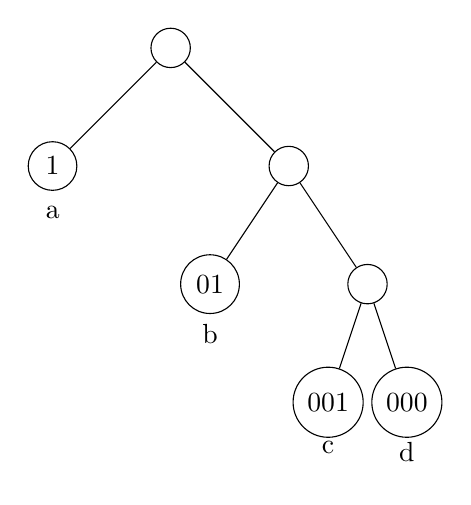
\begin{tikzpicture}[
            level distance=1.5cm,
            level 1/.style={sibling distance=3cm},
            level 2/.style={sibling distance=2cm},
            level 3/.style={sibling distance=1cm},
            every node/.style={circle,draw,minimum size=0.5cm},
            leaf label/.style={draw=none, circle=false, below=0.3cm}
        ]
            \node {}
                child {
                    node {1} 
                    node[leaf label] {a}
                }
                child {
                    node {}
                    child {
                        node {01}
                        node[leaf label] {b}
                    }
                    child {
                        node {}
                        child {
                            node {001}
                            node[leaf label] {c}
                        }
                        child {
                            node {000}
                            node[leaf label] {d}
                        }
                    }
                };
        \end{tikzpicture}
      \end{enumerate}
    \end{example}

    \begin{definition}[Prefix Code]
      Note that all of these encodings except for the nonvalid scheme has the property that no encoding of a character is a prefix of another character. A scheme with this property is called a \textbf{prefix code}. 
    \end{definition}

    \begin{example}
      By modifying the best scheme so far by swapping the $0$s and $1$s, we have 
        \begin{equation}
          C (s) = \begin{cases} 1 & s = a \\ 10 & s = b \\ 100 & s = c \\ 000 & s = d \end{cases}
        \end{equation}
        But this is not a prefix code, though it is a valid code (uniquely decodable since its symmetric counterpart is uniquely decodable). For example, we can sequentially decode the string 
        \begin{equation}
          1000000\ldots 
        \end{equation}
        since we don't know where the $0$s end. While we may be able to decode this if we knew the length, it isn't really easy to decode. 
    \end{example}

    The right intuition as this point is to give characters with large probabilities a short codeword and low ones longer ones. However, this is also not true. 

    \begin{example}
      Let's have the same alphabet but now slightly perturb the probabilities 
      \begin{equation}
        \mathbb{P}(a) = \frac{1}{4} + \epsilon,
        \mathbb{P}(b) = \frac{1}{4} + \frac{\epsilon}{2},
        \mathbb{P}(c) = \frac{1}{4} - \frac{\epsilon}{2},
        \mathbb{P}(d) = \frac{1}{4} - \epsilon,
      \end{equation}
      Then our prefix coding would be 
      \begin{equation}
        C (s) = \begin{cases} 1 & s = a \\ 01 & s = b \\ 001 & s = c \\ 000 & s = d \end{cases}
      \end{equation}
      which still has an expected length of $2.25$, which is not enough to beat just the regular 2-bit encoding of each word. 
    \end{example}

    Here is a better system of thinking about this. If all codewords have length $l$, then the number of codewords that we can make is $2^l$. Then we can think of each codeword of length $l$ having a ``cost'' of $2^{-l}$ in our \textit{codeword supermarket}. 

    \begin{figure}[H]
      \centering 
      \includegraphics[scale=0.4]{img/supermarket.png}
      \caption{Our symbol code supermarket where we can buy code words of length $l$ for a price of $2^{-l}$. Our budget is $1$. } 
      \label{fig:supermarket}
    \end{figure}

    With this visual, there are two constraints that we can reintroduce. First is Kraft's inequality. 

    \begin{theorem}[Kraft Inequality]
      Every viable symbol code must have a budget $\leq 1$. 
      \begin{equation}
        \sum_i 2^{-l_i} \leq 1
      \end{equation}
      If a symbol code achieves equality, then this is called a \textbf{complete symbol code}. 
    \end{theorem}

    Second, a prefix code must have all codewords in different ``rows'' of the supermarket. 

    \begin{figure}[H]
      \centering 
      \includegraphics[scale=0.4]{img/supermarket_prefix.png}
      \caption{A symbol code that is a prefix code. } 
      \label{fig:supermarket_prefix}
    \end{figure}

  \subsection{Huffman Coding}

    Now how well can we do with symbol codes? It turns out that the expected symbol code length cannot beat the entropy, and we will describe how to construct such a symbol code. 

    \begin{theorem}[Ideal Code Lengths]
      Given the expected length of a symbol code $C$ on an ensemble $X$, the expected length cannot be less than the entropy. 
      \begin{equation}
        H(X) \leq \mathbb{E}[\ell(C(X))] = \sum_{s \in \mathcal{S}} \mathbb{P}(s) l_i
      \end{equation}
    \end{theorem}
    \begin{proof}
      Such a code must exist. We first define the \textit{ideal length} of the character $s_i$ with probability $p_i$ to be its surprisal 
      \begin{equation}
        l_i^\ast = \log_2 \frac{1}{p_i} = \sigma_i
      \end{equation}
      If you rearrange this and imagine someone that picked length $l_i$. We can pick an implicit probability $q_i$ satisfying the ideal length.  It is $q_i = 2^{-l_i}$, but the person may not have chosen a complete code, so we must normalize it. 
      \begin{equation}
        q_i = \frac{2^{-l_i}}{Z}
      \end{equation}
      where $Z = 1$ if we have a complete code and $Z < 1$ if not. Therefore, we have 
      \begin{equation}
        l_i = \log_2 \frac{1}{q_i} - \log_2 Z 
      \end{equation}
      We can then plug this into the expected length formula. 
      \begin{align*}
        \mathbb{E}[\ell(C(X))] & = \sum_i p_i \bigg[ \log_2 \frac{1}{q_i} - \log_2 Z \bigg] \\
                               & = \sum_i p_i \log_2 \frac{1}{p_i} + \sum_i p_i \log_2 \frac{p_i}{q_i} - \log_2 Z \\
                               & = H(X) + D_{\mathrm{KL}} (p \mid \mid q) - \log Z \\
                               & \geq H(X)
      \end{align*}
      since the KL divergence (as we will show later) is greater than $0$, and since $Z \leq 1$, we are subtracting a negative number. 
    \end{proof}

    To get equality, the proof shows you that you must make your implicit probabilities equal to your true probabilities, so the length of each character should be equal to its surprisal or information content. But these lengths aren't integers, so we must modify this in practice, which will get close, but not exactly to the true minimum. It turns out that we can get the expected length $L$ such that it is within 1 bit of the true minimum. 
    \begin{equation}
      H(X) \leq L \leq H(X) + 1
    \end{equation}

    This is called the \textit{Huffman algorithm}. 

    \begin{theorem}[Huffman Algorithm]
      The \textbf{Huffman algorithm} constructs an optimal prefix code for a given set of symbols and their probabilities. The algorithm proceeds as follows:

      \begin{enumerate}
        \item Create a leaf node for each symbol, and add it to a priority queue.
        \item While there is more than one node in the queue:
        \begin{enumerate}
          \item Remove the two nodes with the lowest probability from the queue.
          \item Create a new internal node with these two nodes as children, with a probability equal to the sum of their probabilities.
          \item Add the new node back into the queue.
        \end{enumerate}
        \item The remaining node is the root of the Huffman tree.
        \item Traverse the tree, assigning 0 to each left branch and 1 to each right branch.
        \item The Huffman code for each symbol is the sequence of 0s and 1s on the path from the root to that symbol's leaf node.
      \end{enumerate}

      The Huffman algorithm produces an optimal prefix code, meaning that for any given set of symbols and probabilities, no other prefix code produces a smaller expected codeword length.
      \begin{enumerate}
        \item The expected length $L$ of the Huffman code satisfies:
        \begin{equation}
          H(X) \leq L < H(X) + 1
        \end{equation}
        \item The Huffman code is optimal among all prefix codes.
        \item Symbols with higher probabilities get shorter codewords.
        \item The algorithm has a time complexity of $O(n \log n)$ where $n$ is the number of symbols.
      \end{enumerate}
    \end{theorem}

    \begin{example}[Huffman Coding]
      Consider the alphabet $\mathcal{S} = \{A, B, C, D\}$ with probabilities $\{0.4, 0.3, 0.2, 0.1\}$.

      \begin{enumerate}
        \item Initial nodes: A(0.4), B(0.3), C(0.2), D(0.1)
        \item Combine D and C: (D,C)(0.3), A(0.4), B(0.3)
        \item Combine (D,C) and B: ((D,C),B)(0.6), A(0.4)
        \item Final tree: (A,((D,C),B))(1.0)
      \end{enumerate}

      \begin{figure}[H]
        \centering
        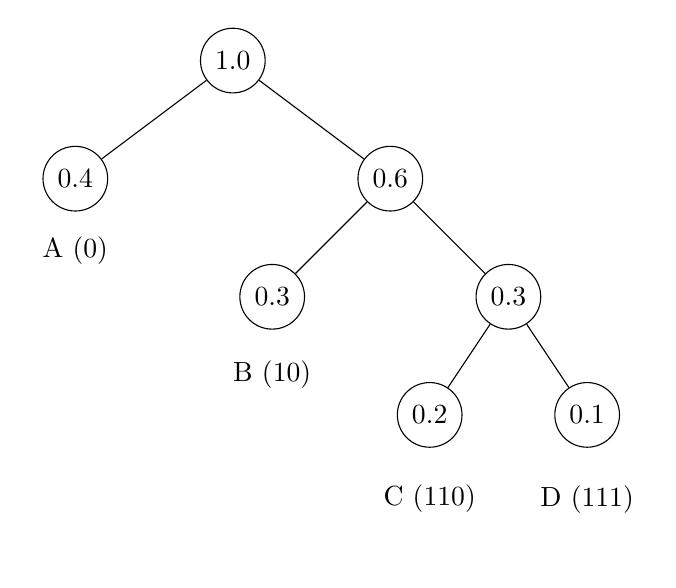
\begin{tikzpicture}[
          level distance=1.5cm,
          level 1/.style={sibling distance=4cm},
          level 2/.style={sibling distance=3cm},
          level 3/.style={sibling distance=2cm},
          every node/.style={circle,draw,minimum size=0.8cm},
          leaf label/.style={draw=none, circle=false, below=0.3cm}
        ]
          \node {1.0}
            child {
              node {0.4} 
              node[leaf label] {A (0)}
            }
            child {
              node {0.6}
              child {
                node {0.3}
                node[leaf label] {B (10)}
              }
              child {
                node {0.3}
                child {
                  node {0.2}
                  node[leaf label] {C (110)}
                }
                child {
                  node {0.1}
                  node[leaf label] {D (111)}
                }
              }
            };
        \end{tikzpicture}
        \caption{Huffman tree for the alphabet $\{A, B, C, D\}$}
        \label{fig:huffman_tree}
      \end{figure}

      Resulting codes:
      \begin{itemize}
        \item A: 0
        \item B: 10
        \item C: 110
        \item D: 111
      \end{itemize}

      The expected length is $L = 0.4(1) + 0.3(2) + 0.2(3) + 0.1(3) = 1.9$ bits compared to the entropy of $H(X) = -\sum_{i} p_i \log_2 p_i \approx 1.85$ bits. This demonstrates that the Huffman code achieves a length very close to the entropy, and always within 1 bit of it:
      \begin{equation}
        H(X) \approx 1.85 \leq L = 1.9 < H(X) + 1 \approx 2.85
      \end{equation}
    \end{example}

  \subsection{Lempel-Ziv (LZ) Compression}

    The \textbf{LZ77} and \textbf{LZ78} (also known as the \textbf{LZ1} and \textbf{LZ2}), respectively, are lossless data compression algorithms published by Lempel and Ziv in 1977/78. They obsolete themselves but form the basis for many modern variations including \textbf{LZW, LZSS, LZMA}, and others. 

    LZ77 and 78 are both dictionary coders, but are not static. Rather, the dictionary starts in some predetermined state but the contents change during the encoding process. 


  \subsection{Data Compression}

    \textbf{Data compression}, also called \textbf{source coding} or  \textbf{bit-rate reduction}, is the process of encoding information using fewer bits than the original representation. Data compression algorithms can be categorzied into two types: 
    \begin{enumerate}
        \item \textbf{Lossless compression} reduces bits by identifying and eliminating statistical redundancy. No information is lost in lossless compression. 
        \item \textbf{Lossy compression} reduces bits by removing unnecessary or less important information.
    \end{enumerate}
    Typically, a device that performs data compression is referred to as an \textbf{encoder}, and one that performs the reversal of the process (decompression) as a \textbf{decoder}. 

    A \textbf{space–time} or \textbf{time–memory trade-off} in computer science is a case where an algorithm or program trades increased space usage with decreased time. Here, space refers to the data storage consumed in performing a given task (RAM, HDD, etc), and time refers to the time consumed in performing a given task (computation time or response time). 

    A space–time trade-off can be applied to the problem of data storage. If data is stored uncompressed, it takes more space but access takes less time than if the data were stored compressed (since compressing the data reduces the amount of space it takes, but it takes time to run the decompression algorithm). Depending on the particular instance of the problem, either way is practical. There are also rare instances where it is possible to directly work (which may also be faster) with compressed data. 

    \subsection{Data Compression Ratio}
    The \textbf{data compression ratio}, also known as the \textbf{compression power}, is a measurement of the relative reduction in size of data representation produced by a data compression algorithm. It is defined as 
    \[\text{Compression Ratio} = \frac{\text{Uncompressed Size}}{\text{Compressed Size}}\]
    For example, a representation that compresses a file's storage size from 10MB to 2MB has a compression ratio of $10/2 = 5$. We can alternatively talk about the \textbf{space saving}, which is defined
    \[\text{Space Saving} = 1 - \frac{\text{Compressed Size}}{\text{Uncompressed Size}}\]
    So, the previous representation yields a space saving of 0.8, or $80\%$. 

    Lossless compression of digitized data such as video, digitized film, and audio preserves all the information, but it does not generally achieve compression ratio much better than 2:1 because of the \textbf{intrinsic entropy} of the data. Compression algorithms which provide higher ratios either incur very large overheads or work only for specific data sequences (e.g. compressing a file with mostly zeros). In contrast, lossy compression (e.g. JPEG for images, or MP3 and Opus for audio) can achieve much higher compression ratios at the cost of a decrease in quality, such as Bluetooth audio streaming, as visual or audio compression artifacts from loss of important information are introduced. In general, whether a compression ratio is high or not really depends on what kind of data is being compressed and how it is compressed. 


    \subsection{Lossless Compression}
    Lossless data compression algorithms usually exploit statistical redundancy to represent data without losing any information, so that the process is reversible. Lossless compression is possible because most real-world data exhibits statistical redundancy. For example, an image may have areas of color that do not change over several pixels; instead of coding "red pixel, red pixel, ..." the data may be encoded as "279 red pixels". This is a basic example of run-length encoding; there are many schemes to reduce file size by eliminating redundancy.

    A \textbf{dictionary coder}, also known as a \textbf{substitution coder}, is a class of lossless data compression algorithms which operate by searching for matches between the text to be compressed and a set of strings contained in a data structure (called the 'dictionary') maintained by the encoder. When the encoder finds such a match, it substitutes a reference to the string's position in the data structure. 

    Some dictionary coders use a \textit{static dictionary}, one whose full set of strings is determined before coding begins and does not change during the coding process. This approach is most often used when the message or set of messages to be encoded is fixed and large; for instance, an application that stores the contents of a book in the limited storage space of a PDA generally builds a static dictionary from a concordance of the text and then uses that dictionary to compress the verses. 

    In a related and more general method, a dictionary is built from redundancy extracted from a data environment (various input streams) which dictionary is then used statically to compress a further input stream. For example, a dictionary is built from old English texts then is used to compress a book. More common are methods where the dictionary starts in some predetermined state but the contents change during the encoding process, based on the data that has already been encoded. 

    \subsubsection{Run-length Encoding (RLE) Compression}
    RLE is a form of lossless data compression in which \textit{runs} of data (sequences in which the same data value occurs in many consecutive data elements) are stored as a single data value and count, rather than as the original run. This is most useful on data that contains many such runs.

    For example, consider a screen containing plain black text on a solid white background. There will be many long runs of white pixels in the blank space, and many short runs of black pixels within the text. A hypothetical scan line, with B representing a black pixel and W representing white, might read as follows: 
    \begin{lstlisting}
    WWWWWWWWWWWWBWWWWWWWWWWWWBBBWWWWWWWWWWWWWWWWWWWWWWWWBWWWWWWWWWWWWWW
    \end{lstlisting}
    With a RLE data compression algorithm applied to the above hypothetical scan line, it can be rendered as follows: 
    \begin{lstlisting}
    12W1B12W3B24W1B14W
    \end{lstlisting}
    which can be interpreted as a sequence of 12 Ws, 1 B, 12 Ws, 3 Bs, and so on. This run-length code represents the original 67 characters in only 18. While the actual format used for the storage of images is generally binary rather than ASCII characters like this, the principle remains the same. Even binary data files can be compressed with this method. 

